\documentclass[twocolumn]{rbef}
\usepackage{lipsum}

\usepackage{bbm}
\usepackage{subfig}
\usepackage{pdfpages} % Para incluir a capa.

\newcommand{\1}{\mathbbm{1}}
\newcommand{\s}{\mathcal{S}}
\newcommand{\T}{\mathcal{T}}
\newcommand{\A}{\mathcal{A}}
\newcommand{\ket}{\rangle}
\newcommand{\bra}{\langle}

\newtheorem{defi}{Definição}
\newtheorem{theorem}{Teorema}
\newtheorem{acknowledgement}[theorem]{Acknowledgement}
\newtheorem{algorithm}[theorem]{Algorithm}
\newtheorem{axiom}[theorem]{Axiom}
\newtheorem{claim}[theorem]{Claim}
\newtheorem{conclusion}[theorem]{Conclusion}
\newtheorem{condition}[theorem]{Condition}
\newtheorem{conjecture}[theorem]{Conjecture}
\newtheorem{corollary}[theorem]{Corollary}
\newtheorem{criterion}[theorem]{Criterion}
\newtheorem{definition}[theorem]{Definition}
\newtheorem{example}[theorem]{Example}
\newtheorem{exercise}[theorem]{Exercise}
\newtheorem{lemma}[theorem]{Lemma}
\newtheorem{notation}[theorem]{Notation}
\newtheorem{problem}[theorem]{Problem}
\newtheorem{proposition}[theorem]{Proposition}
\newtheorem{remark}[theorem]{Remark}
\newtheorem{solution}[theorem]{Solution}
\newtheorem{summary}[theorem]{Summary}
\newenvironment{proof}[1][Proof]{\noindent\textbf{#1.} }{\ \rule{0.5em}{0.5em}}

\titulocabecalho{Comportamento do cliente: estudo de caso de uma empresa prestadora de serviços de contabilidade digital}
\autorcabecalho{A. H. A. Rafael}

\numeracao{01}
\volume{01}
\numero{01}
\ano{2020}
\doi{http://dsbd.leg.ufpr.br/tcc}
% \tipodeartigo{TCC DSBD}
\tipodeartigo{Especialização em Data Science \& Big Data}
% \addtocounter{page}{566} %% \setcounter produces extra white page!!! use ===\addtocounter===
\begin{document}

\author[1]{Aphonso H. A. Rafael}\href{emailto:aphonsoarafael@gmail.com}

\affil[1]{Departamento de Estatística, Universidade Federal do Paraná.}

\titulo{Comportamento do cliente: estudo de caso de uma empresa prestadora de serviços de contabilidade digital}

% \subtitulo{vazio}

% -----------------------------------------------------------------------

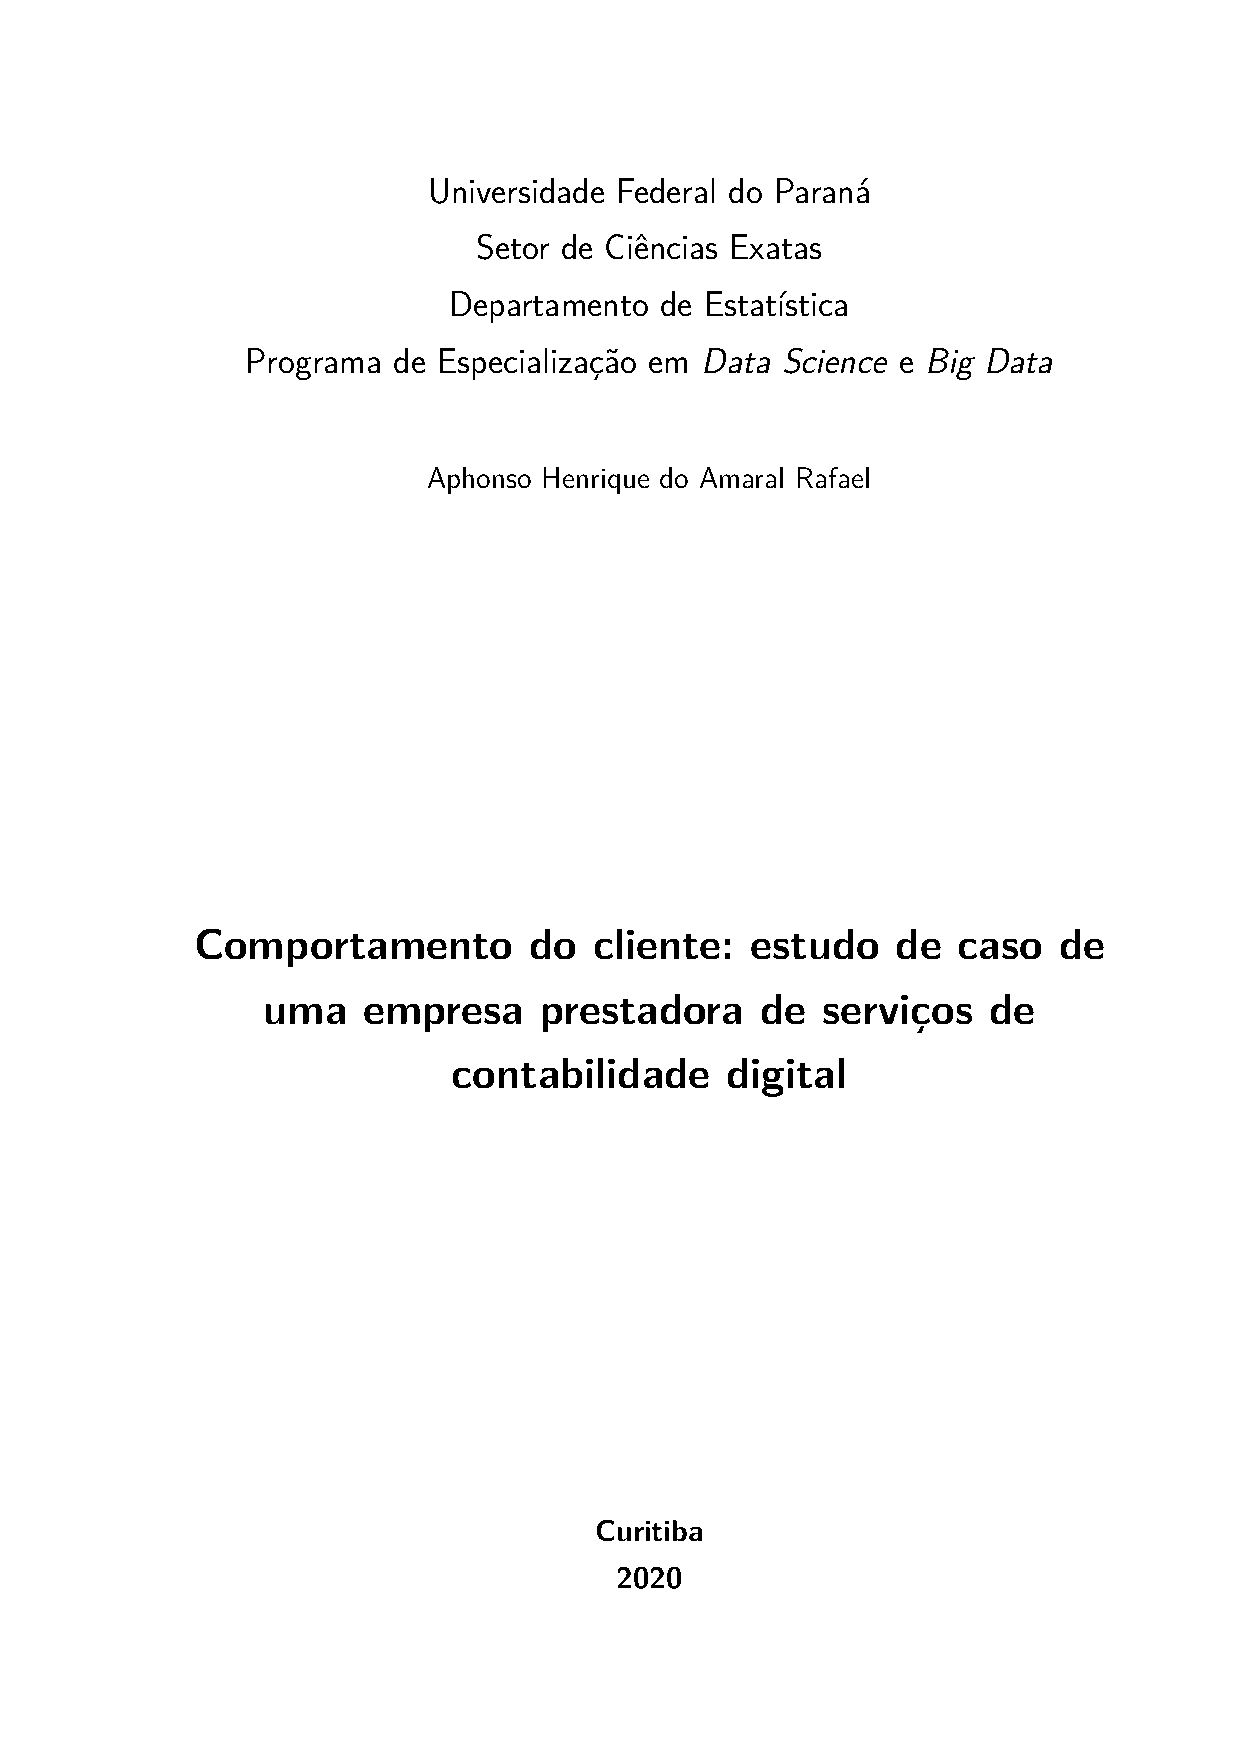
\includepdf[pages=-]{Capa.pdf} % Incluí a capa

\begin{primeirapagina}

\begin{abstract}
Esta pesquisa se propõe a ser um primeiro passo num projeto maior de \emph{customer success} (sucesso do cliente), numa empresa que presta serviços de contabilidade digital, é um estudo de caso a partir do atual cenário da empresa. Acredita-se que, através de dados e técnicas de \emph{machine learning}, podem ser extraídas informações e \emph{insights} importantes que direcionem projetos, ações e a tomada de decisão, implicando numa melhor prestação do serviço e a melhoria da experiência do cliente. Com os resultados, a empresa ganha material para análises exploratórias e descobertas no desenvolvimento de seus objetivos. Empresas jovens, em modelos de negócio inovadores/disruptivos, carecem de modelos ou \emph{benchmarks} de atuação, pois praticamente não há pares ou experiências similares no mercado. Através dos resultados desta pesquisa, foi possível identificar que há distinção entre os perfis de clientes, como também na forma como estes perfis interagem com a empresa. Sob este contexto, a pesquisa sugere uma metodologia para análise de dados do perfil dos clientes, bem como na forma e no porque estes interagem com a empresa, possibilitando elaborar ações, seja de processos ou tecnologia, que melhorem a experiência como um todo.
\palavraschave{contabilidade digital, perfil de cliente, atendimento, service-desk, experiência ao cliente}.
\end{abstract}

\begin{otherlanguage}{english}
\begin{abstract}
This research proposes to be a first step in a larger project of customer success, in a company that provides digital accounting services. It is a case study from its current scenario. Inside the company, staff believe that through data and machine learning techniques, they could get important insights and information that could guide projects, actions plans and support the decision making process, which might help company to provide better services and improve customer experience. From obtained results, company gets material for further exploratory analysis and discover new ways to develop its objectives. Young companies, that operate in innovative and disruptive business models, have a lack of benchmarks to follow or inspire themselves, as there are practically no peers or similar experiences in this market. Through the results of this research, it was possible to identify there are differences between customer profiles, as well in the way they interact with the company. In this context, this research suggests a methodology for analyzing customer profile data and how they interact with the company. Through this, the company is able to develop new actions, either on processes or technology, that could improve the full customer experience.
\keywords{digital accounting, customer profile, customer service, service-desk, customer experience}.
\end{abstract}
\end{otherlanguage}

\end{primeirapagina}

\section{Introdução}

A contabilidade é uma ciência antiga e que permanece em constante evolução, com registros anteriores ao nascimento de Cristo até os dias atuais. A base da contabilidade moderna, utilizada em todas as empresas do mundo, é conhecida como o “Método das Partidas Dobradas” (SCHIMIDT, 2008)\cite{SCHMIDT}. Negra (2003, p. 1)\cite{NEGRA} destaca que “o Método das Partidas Dobradas foi exposto, oficialmente, por Luca Pacioli em 1494, em sua obra Suma de Aritmética, Geometria, Proporção e Proporcionalidade”; ainda que a autora também destaque e demonstre que o método é anterior a Pacioli, existindo registros históricos ainda anteriores ao século XVI (NEGRA, 2003)\cite{NEGRA}.
\newline Como cita Imperatore (2017)\cite{IMPERATORE} a contabilidade é tratada como uma ciência social, cujo objetivo é estruturar um sistema de avaliação e fornecimento de informações, a fim de “[...] prover seus usuários com relatórios, demonstrações e análises de natureza econômico-financeira da empresa em determinado momento, bem como sua evolução em determinado período” (IMPERATORE, 2017, p. 12)\cite{IMPERATORE}. Ainda que evidentemente antiga, a contabilidade é um assunto técnico e pouco compreendido por quem não é, necessariamente, um estudioso da área ou frequente usuário dos seus métodos, processos e relatórios. 
\newline Com a aceleração digital que o mundo vem enfrentando em todos os segmentos, os serviços contábeis também vem passando por muitas mudanças, seja na forma como é prestado, até mesmo em como o empresário lida com suas rotinas contábeis. É neste contexto que começam a surgir no Brasil, empresas especializadas na prestação deste serviço de maneira totalmente online, denominadas de “Contabilidade Digital”. No Brasil, a partir de 2013 este movimento passou a ganhar força com o “[...] uso da tecnologia para automatizar processos e rotinas na regularização das contas das empresas” (ISTOÉ DINHEIRO, 2020)\cite{ISTOE}.
\newline Não apenas no contexto de prestação de serviços contábeis de maneira digital, estas empresas também têm sido importantes responsáveis no acesso e democratização à formalização de novos negócios, antes informais (sem registro, CNPJ, etc) e também ao facilitar a abertura de novas empresas; formalizando atividades de diversos tipos de empreendedores (ISTOÉ DINHEIRO, 2020)\cite{ISTOE}; sobretudo as de pequeno porte que, em 2008, eram mais de 10 milhões de empreendimentos no Brasil, sendo 98\% deles informais (EXAME, 2008)\cite{EXAME}.
\newline Nesse cenário, esta pesquisa é um estudo de caso de uma das principais empresas de Contabilidade Digital em atuação no Brasil, que é um mercado é novo, tanto para os usuários, quanto para a própria empresa - que também tem poucos anos de existência e é vetor deste novo paradigma. Por isso, diversas questões precisam ser analisadas e discutidas, para que a empresa possa entregar uma experiência cada vez melhor aos clientes, assim como aprimorar seus processos internos, alocação de recursos, produto e a combinação de pessoas e tecnologia, para alavancar sua eficiência, crescimento e perenidade.


\section{Contextualização e motivação} \label{Sessao2}

Como citado, a contabilidade é um assunto complexo e muitas vezes subjetivo até mesmo para quem é da área. Micro e pequenos empresários, usuários dos serviços de Contabilidade Digital (e novos empreendedores) não costumam dominar o tema. Por isso, acredita-se que existem diversos tipos de empresas e negócios e, para cada um deles, dúvidas e necessidades/demandas distintas em sua jornada.
\newline Pragmaticamente, por esta pesquisa busca-se encontrar um caminho para oferecer uma proposta de valor diferenciada aos clientes da empresa, que vá ao encontro de suas necessidades, conforme a demanda que eles possuem, ou seja, num viés de personalização da prestação do serviço conforme o tipo do cliente e o que ele busca. 
Para tal, a pesquisa foi estruturada em 3 grandes etapas: 
\newline\textbf{1.} Conhecimento, por parte da empresa, de quem são seus clientes (quais são os tipos/perfis);  
\newline\textbf{2.} Conhecer os tipos de demanda que seus clientes possuem; isto é: quando o cliente precisa interagir com o atendimento da empresa (\emph{service-desk}); que tipo de demandas eles buscam; 
\newline\textbf{3.} A partir dos resultados obtidos nos itens 1 e 2; analisar os perfis Vs. demandas para compreender as diferenças de comportamentos e necessidades dos clientes em sua jornada. 
Espera-se que, a partir dos resultados, a empresa possa encontrar respostas e elaborar ações, seja de melhoria de processos, como de produto ou tecnologia, para aprimorar a experiência do cliente e sua alavancagem, escala.


\section{Metodologia e bases de dados} \label{Sessao3}

Para cada uma das etapas, foram utilizadas técnicas distintas de análise de dados, uma vez que buscavam endereçar questões diferentes.
Todos os dados utilizados são da própria companhia, extraídos pelo autor dos bancos de dados, por meio de consultas em \emph{SQL}. Uma vez que aqui são tratados dados de clientes e, em alguns casos, sigilosos, buscou-se priorizar análises agregadas e preservar a confidencialidade.
\newline\textbf{Etapa 1}: a empresa possui hoje mais de 20 mil clientes, evidentemente, não há como analisá-los - ou imaginar uma prestação de serviço customizada - de forma individual, por isso, o objetivo foi agrupar (clusterizar) estes clientes e identificar os perfis, semelhanças e diferenças. Uma vez que também não se sabia o número de possíveis perfis dentre essa massa de clientes, foram utilizadas técnicas de \emph{machine learning}, por meio de Agrupamento Hierárquico e análise de dendrograma. Após identificar o número de \emph{clusters}, utilizou-se o \emph{K-Means} para agrupamento e nova avaliação dos resultados e análise das variâncias explicadas a partir do números de \emph{clusters}, pelo \emph{Elbow Method}. As \emph{features} consideradas para tal foram selecionadas pelo autor, conforme critérios negociais da empresa, isto é, incluindo no modelo variáveis que do ponto de vista de negócio poderiam influenciar nos tipos de demandas/necessidades dos clientes, durante sua jornada.
\newline\textbf{Etapa 2}: buscou-se compreender os tipos de demandas que os clientes possuem com os serviços prestados. Existem dois canais para atendimento (no \emph{service-desk}) com a empresa, ambos são por escrito e inteiramente registrados: i) abertura de chamados (tickets), via troca de mensagens por email e ii) abertura de atendimento instantâneo via troca de mensagens (chat).
O \emph{service-desk} é segmentado em três níveis: 1) nível 1: topo do funil de atendimentos, isso é, a entrada de todo tipo de dúvida e de cliente. Aqui são atendidas dúvidas mais simples, de usabilidade do sistema ou rotinas básicas do cliente. 2) segundo nível, onde chegam dúvidas técnicas mais complexas, como questões legais, tributárias, ou para tipos de negócio/clientes específicos, que precisam de análise profissional detalhada e tomada de decisão. 3) o nível 3, por fim, refere-se a prestação de serviços, como alterações de documentos, reabertura de balanços, consultoria paga (legal e tributária), ajustes contábeis ou demais atividades que extrapolam os serviços básicos cobertos no contrato. Os atendimentos dos níveis Avançado e Premium (cfe. seção \ref{Sessao4.2.1}) agregam os níveis 1 e 2 numa única célula de atendimento, porém somente para os clientes que aderem a estes planos.
Desta forma, foi selecionada uma base de dados contendo os atendimentos realizados nos níveis 1, 2, 3, Avançado e Premium, durante o período de sete meses (janeiro a julho de 2020). O total de itens analisados (tickets + chats) foi de aproximadamente 77 mil atendimentos e, nesta base, foram utilizadas técnicas de \emph{machine learning} para mineração de texto (MinTex) / processamento de linguagem natural \emph{(Natural Language Processing - NLP)}. Em sequência, foram treinados e testados modelos de classificação a partir de uma base rotulada de 383 itens - que foi classificada pela empresa para esta pesquisa - categorizando estes atendimentos entre as opções i) dúvida; ii) problema; iii) solicitação e, por fim, foram preditos/classificados os atendimentos.
\newline\textbf{Etapa 3}: a partir dos resultados dos itens 1 e 2; foram realizadas análises exploratórias e estatísticas descritivas. Na sequência, os resultados dos itens 1 e 2 foram combinados para identificar macro-comportamentos, com o objetivo de prover então à empresa, os \emph{insights} propostos nesta pesquisa.
Devido ao grande volume de dados, o processamento dos algoritmos e análises foram realizados em uma nuvem fornecida pela própria empresa, em ambiente GCP (\emph{Google Cloud Platform}). A configuração da máquina foi uma \emph{Virtual Machine standard} do GCP (\emph{n1-highmem-16}); cuja infraestrutura é composta de 16 vCPUs com 104 GB de memória e sistema operacional Debian.
As modelagens, técnicas estatísticas e de \emph{machine learning} foram executadas na linguagem \emph{Python}, versão base 3.8; por meio das principais bibliotecas utilizadas para essas finalidades, tais como Scikit-Learn, SciPy, NLTK e as clássicas bibliotecas de manipulação e visualização de dados como Pandas, Numpy, Matplotlib e Seaborn.
Os códigos, assim como os requerimentos com o detalhamento das bibliotecas e versões (\texttt{requirements.txt}), estão disponibilizados no \href{https://github.com/aphonsoar/Data-Science-Big-Data-UFPR}{\emph{Github}}\footnote{\url{https://github.com/aphonsoar/Data-Science-Big-Data-UFPR}}.


\section{Experimentos e análise dos resultados} \label{Sessao4}
\subsection{Clusterização de clientes} \label{Sessao4.1}

O \emph{dataset} com dados dos clientes foi elaborado de maneira em que cada linha representa um CNPJ (ou seja, uma empresa) e as colunas são as \emph{features} (variáveis) para clusterização. Originalmente, ele possuía além da chave (CNPJ) outras 17 variáveis, sendo 10 numéricas e 7 categóricas. Uma vez que não é trivial realizar agrupamento por variáveis categóricas, foi necessária uma etapa de pré-processamento de dados, transformando estas variáveis categóricas em numéricas (SARKAR, 2019)\cite{SARKAR}. Convencionalmente, duas técnicas são principalmente utilizadas para tal: i) Label Encoder e ii) One Hot Encoding (SHAIKH, 2018)\cite{SHAIKH}:\newline
%--------------------------------------------------------------------------------
\newline\textbf{i) Label Encoder:} define as variáveis categóricas em números inteiros entre 0 e $N$ ($nclasses - 1$), onde $N$ é o número de classes distintas. Se a classe se repete, o mesmo número inteiro é atribuído a todas as repetições. \textbf{Limitações:} como os valores das variáveis categóricas passam a ser de 0 a $N$, isso cria uma impressão de relacionamento e continuidade para o modelo, ou seja, que a classe 1 é menor que a 2, a 2, menor que a três e assim sucessivamente: $1 < 2 < 3 < N$ (relação ordinal).
%--------------------------------------------------------------------------------
\linebreak\textbf{ii) One Hot Encoding:} segrega as variáveis categóricas entre seus valores, atribuindo um valor binário, ou seja: será criada uma coluna para cada classe, de cada variável categórica, é definido o valor zero ou um (0 ou 1) para essa coluna, sendo 1 verdadeiro e 0 falso. \textbf{Limitações:} como cada classe, de cada variável categórica, é transformada numa coluna na base de dados, o que pode aumentar consideravelmente o número de atributos do \emph{dataset} (colunas na base), fazendo com que se amplie o risco de \emph{Maldição da Dimensionalidade}.
%--------------------------------------------------------------------------------
\newline\linebreak Após testes realizados com ambos os métodos, optou-se, finalmente, pelo segundo: (\emph{One Hot Encoding}), pois o número de colunas não aumentou de forma a impactar nos graus de liberdade ou causar Maldição da Dimensionalidade; além de que o outro método criaria a relação ordinal entre os valores das variáveis, influenciando na clusterização. Com isso, o \emph{dataset} passou ter 49 \emph{features}, sendo as mesmas 10 numéricas e 39 categóricas. Na figura \ref{fig1} é possível verificar a composição do \emph{dataset}. Em \emph{vermelho} estão destacadas as variáveis categóricas e em \emph{azul} as numéricas. Apenas uma das colunas apresentou \emph{missing values}: [Idade\_media\_socios]. Estes registros eram cerca de 9\% dos itens e foram ignorados na clusterização.
%--------------------------------------------------------------------------------
\begin{figure}[!htb]
  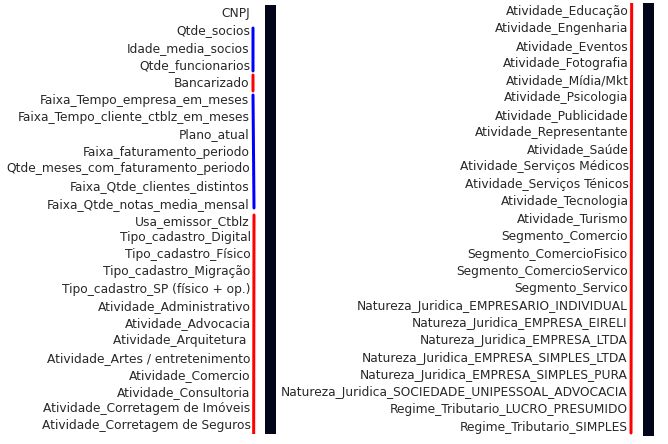
\includegraphics[scale=0.5]{1. Dataset clientes - variaveis.png}
  \caption{Dataset clientes: features consideradas}
  \label{fig1}
\end{figure}
%--------------------------------------------------------------------------------
\newline\linebreak Formalmente, o método do Agrupamento Hierárquico parte da base de dados, isto é, todos os $N$ itens do \emph{dataset} (todos os clientes) formando $N$ \emph{clusters}, onde $N$ é o número de clientes. A partir dos $N$ \emph{clusters}, o algoritmo encontra os 2 pontos mais próximos entre si, através do cálculo da distância euclidiana ($N_x$; $N_y$) e cria um novo \emph{cluster} agregando estes 2, num processo aglomerativo. O processo é seguido sucessivamente até que todos os valores se tornem 1 único \emph{cluster}. Este processo é representado, portanto, pelo gráfico de dendrograma, onde é possível visualizar os níveis de cada nó da agregação e definir qual o melhor número de $k$, onde \emph{k = nº clusters}. 
Neste agrupamento foi utilizado o Método de Ward, que se consiste num “[...] procedimento de agrupamento hierárquico no qual a medida de similaridade usada para juntar agrupamentos é calculada como a soma de quadrados entre os dois agrupamentos feita sobre todas as variáveis” (SEIDEL et al., 2008, p. 10)\cite{SEIDEL}. O método é representado pela equação abaixo e utiliza um algoritmo de minimização de variâncias, que “[...] tende a resultar em agrupamentos de tamanhos aproximadamente iguais” (SEIDEL et al., 2008, p. 10)\cite{SEIDEL}.
%--------------------------------------------------------------------------------
\begin{align*}
d(u, v) = \sqrt{\frac{|v| + |s|}{T} d(v, s)^2 + \frac{|v| + |t|}{T} d(v, t)^2 - \frac{|v|}{T} d(s, t)^2}
\end{align*}
%--------------------------------------------------------------------------------
Na equação, \emph{u} é o novo \emph{cluster} aglomerado a partir dos \emph{clusters} \emph{s} e \emph{t}. Por sua vez, \emph{v} é um \emph{cluster} não utilizado na floresta \emph{T = |v| + |s| + |t|}, e o fator de multiplicação \emph{|*|} é a cardinalidade desses argumentos. Isso também é conhecido como algoritmo incremental (SCIPY, 2020)\cite{SCIPY}. Os resultados obtidos podem ser vistos nas figuras \ref{fig2} e \ref{fig3} (Dendrograma e \emph{Elbow Method Chart}).
%--------------------------------------------------------------------------------
\begin{figure}[!htb]
  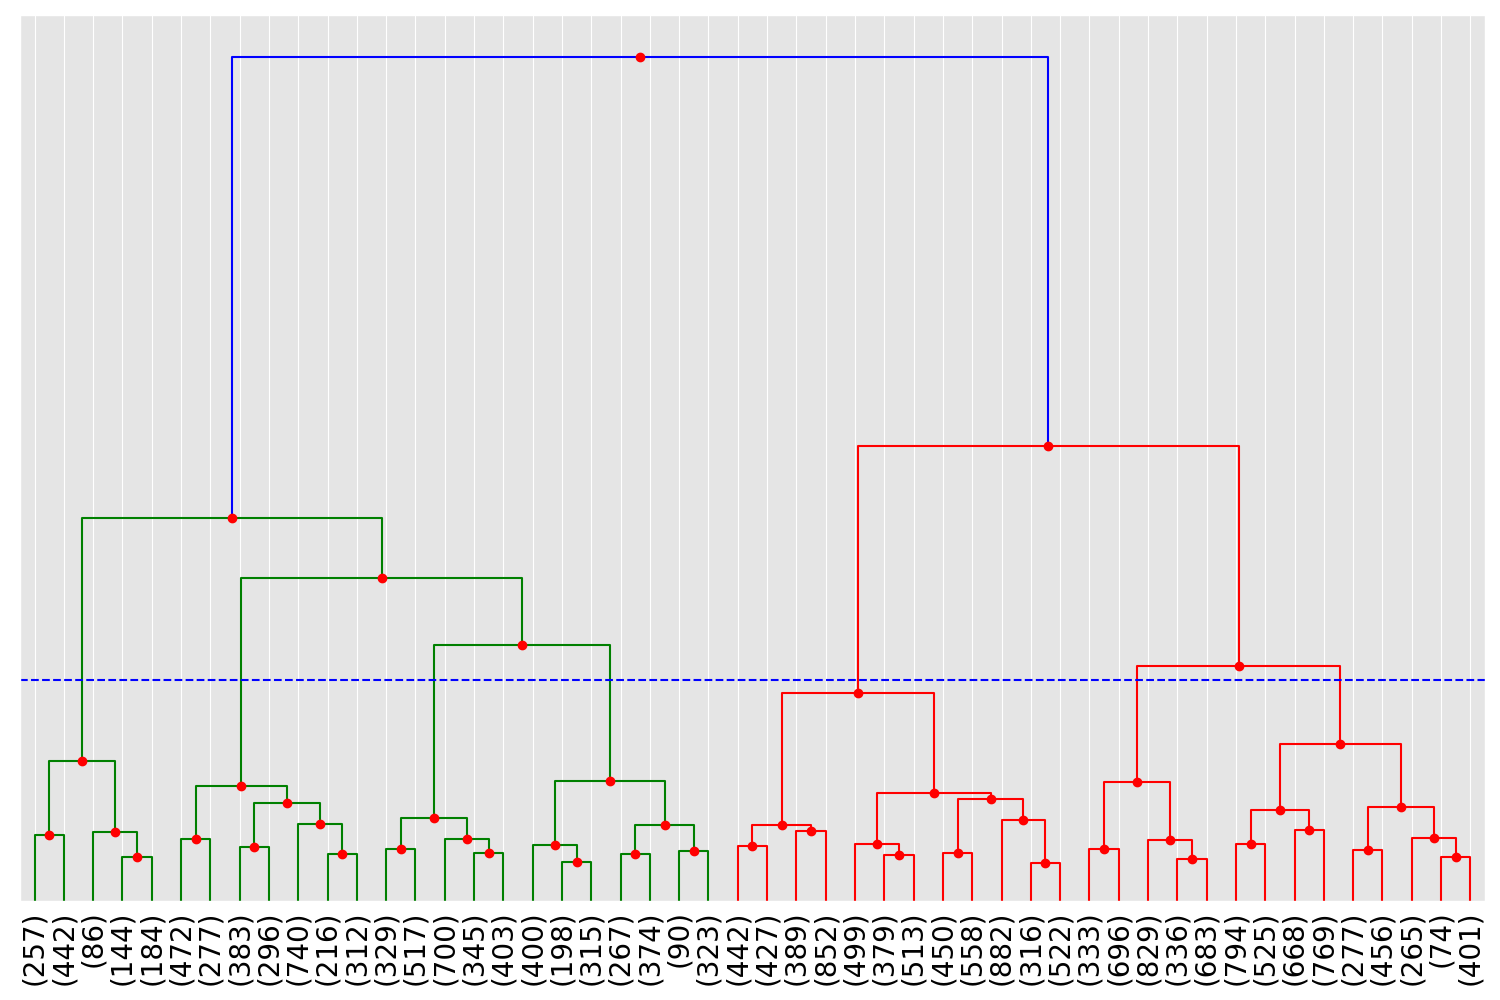
\includegraphics[scale=0.22]{2. Dendrograma Clientes 7 clusteres.png}
  \caption{Dendrograma com últimos 50 nós}
  \label{fig2}
\end{figure}
%--------------------------------------------------------------------------------
%--------------------------------------------------------------------------------
\begin{figure}[!htb]
  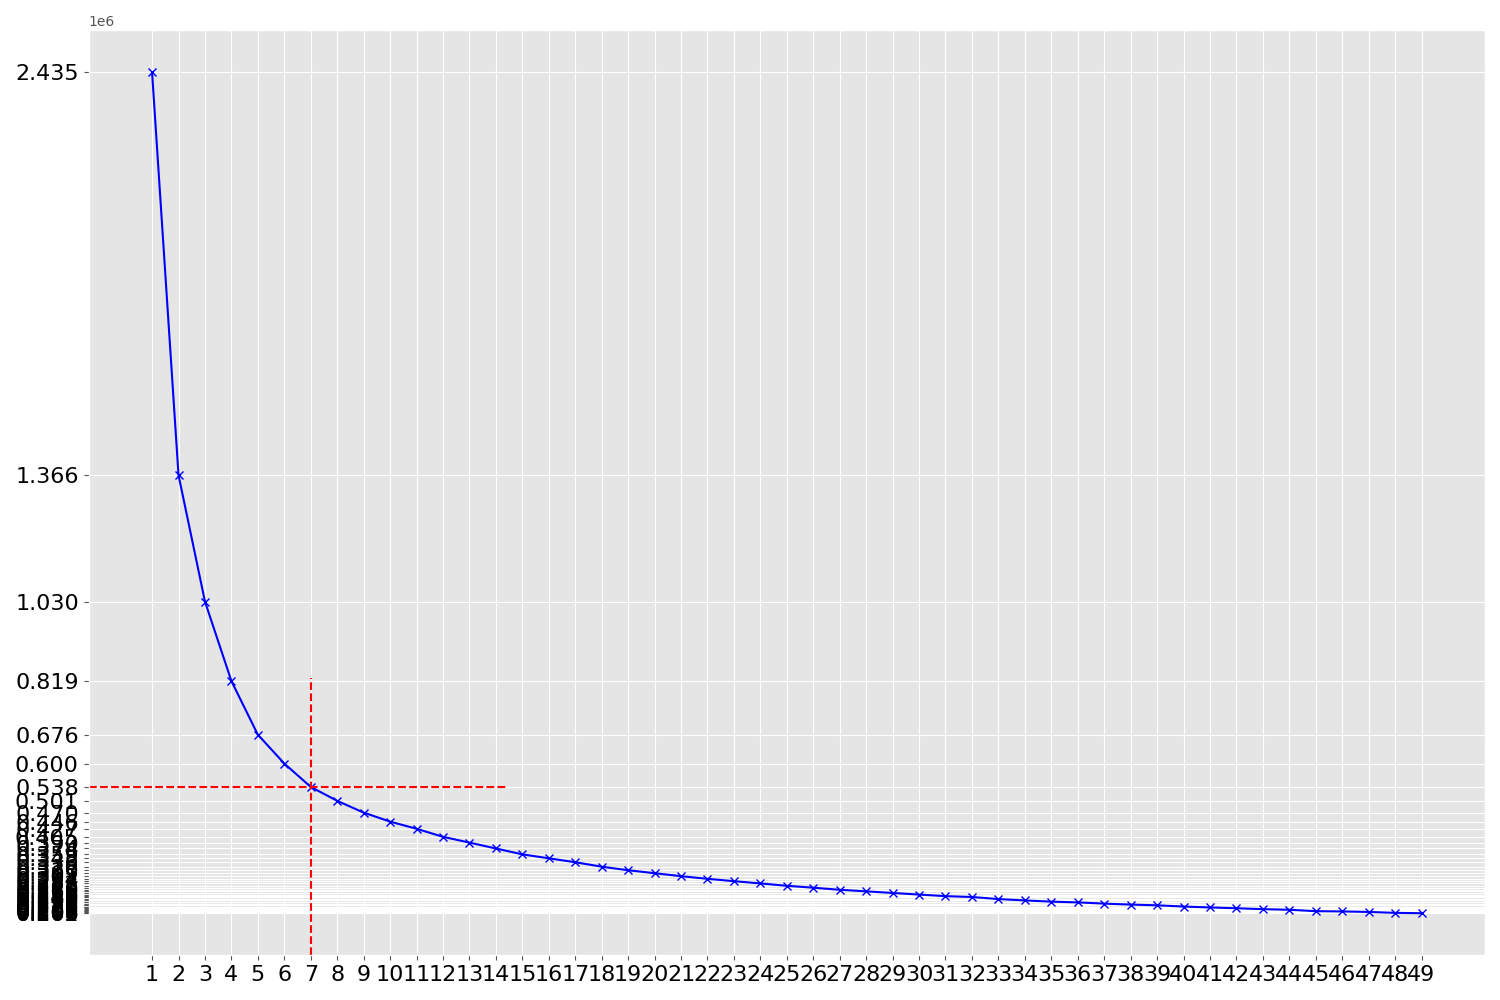
\includegraphics[scale=0.22]{3. Elbow - Clientes 7 clusteres.png}
  \caption{Gráfico do Elbow Method cortado em 7 clusters}
  \label{fig3}
\end{figure}
%--------------------------------------------------------------------------------
\newline\linebreak Conforme análise do Dendrograma e também pelo ponto de inflexão do gráfico do \emph{Elbow Method}, definiu-se portanto, a clusterização dos clientes em 7 grupos, distribuídos conforme figura \ref{fig4}.
%--------------------------------------------------------------------------------
\begin{figure}[!htb]
  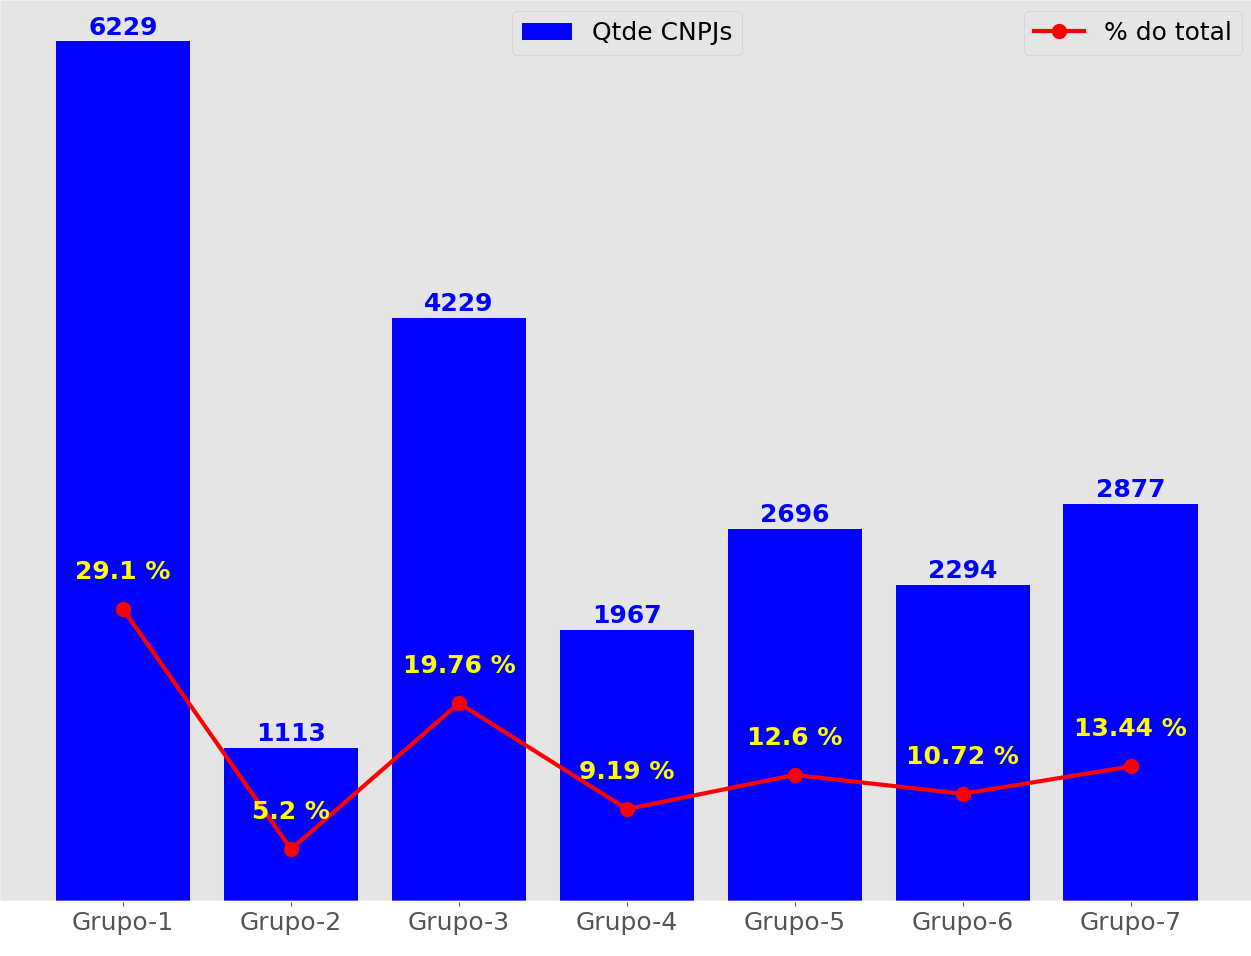
\includegraphics[scale=0.26]{4. Distribuição_CNPJs_clusters_7.png}
  \caption{Distribuição dos clientes entre os clusters}
  \label{fig4}
\end{figure}
%--------------------------------------------------------------------------------
%--------------------------------------------------------------------------------
\subsection{Classificação e predição dos atendimentos} \label{Sessao4.2}
\subsubsection{Pré-processamento e análise exploratória} \label{Sessao4.2.1}
Para análise dos atendimentos, foram construídos inicialmente dois \emph{datasets}: i) tickets (emails) e ii) chats. Para ambos, todo o histórico de troca de mensagens entre o operador e o cliente foram concatenados em uma única \emph{string} e em seguida os \emph{datasets} foram unidos em uma base única. Quando se trabalha com \emph{MinTex} e \emph{NLP} também é importante realizar pré-processamento dos dados para que as \emph{strings} / sentenças possam oferecer melhores condições preditoras (BOEHMKE, 2020)\cite{BOEHMKE}. Este pré-processamento foi realizado nas seguintes etapas:
%--------------------------------------------------------------------------------
\newline\linebreak\textbf{i) normalização do texto:} a) palavras convertidas para \emph{lowercase} (uma vez que os algoritmos são \emph{case sensitive}); b) removidos os símbolos e pontuações; c) removidos espaços vazios (em branco) em excesso e; d) removidos os números (0 a 9) das \emph{strings}.
%--------------------------------------------------------------------------------
\newline\linebreak\textbf{ii) \emph{stopwords}:} são palavras que não possuem significado sintático e não colaboram com informações relevantes numa sentença, seja no sentido ou compreensão da frase, como também poderão atrapalhar ou confundir o algoritmo. São palavras como: “e”, “ou”, “para”, “de” e similares, preposições e termos de ligamento; por isso é recomendado sua remoção (SARKAR, 2019)\cite{SARKAR}. A biblioteca NLTK possui uma lista de \emph{stopwords} em diversos idiomas, entre elas o Português. Foi utilizada esta lista \emph{default} com o incremento de mais algumas centenas de palavras pelo autor, conforme contexto do texto e da análise, totalizando 557 \emph{stopwords}.
%--------------------------------------------------------------------------------
\newline\linebreak Uma vez que o volume de atendimentos analisados está na casa das dezenas de milhares, é evidente imaginar que existe uma infinidade de palavras distintas utilizadas em todas estas trocas de mensagens, por isso, inicialmente foi feita uma análise exploratória das palavras usadas, onde \emph{insights} importantes foram extraídos.
%--------------------------------------------------------------------------------
\newline\linebreak Por meio da da biblioteca NLTK, foi utilizado um algoritmo para “tokenizar” cada palavra que aparece em cada um dos atendimentos, isto é, fazer uma uma contagem de quantas vezes cada palavra se repete em todas as sentenças. A partir disso, podemos analisar sua frequência e distribuição.
%--------------------------------------------------------------------------------
\begin{table}[!htb]
\caption{Frequência das primeiras 10 palavras}
\label{tab1}
\resizebox{\columnwidth}{!}{%
\begin{tabular}{c*{5}{>{$}c<{$}}}
& \text{\textbf{Palavra}} & \text{\textbf{Frequência}} & \text{\textbf{Percentual}} & \text{\textbf{Percentual acumulado}} \\
1 & empresa & 108.261 & 0,01133 & 0.01133 \\
2 & labore & 88.762 & 0,00929 & 0.02062 \\
3 & valor & 85.508 & 0,00895 & 0.02957 \\
4 & contabilidade & 76.612 & 0,00802 & 0.03759 \\
5 & pró & 69.460 & 0,00727 & 0.04487 \\
6 & sucesso & 65.750 & 0,00688 & 0.05175 \\
7 & plataforma & 65.461 & 0,00685 & 0.05860 \\
8 & mês & 60.816 & 0,00636 & 0.06497 \\
9 & pagamento & 60.387 & 0,00632 & 0.07129 \\
10 & nota & 55.804 & 0,00584 & 0.07713 \\
\end{tabular}}
\end{table}
%--------------------------------------------------------------------------------
\newline\linebreak Na tabela \ref{tab1}, constam as primeiras 10 palavras que mais apareceram nos textos dos atendimentos, verifica-se que a palavra que mais apareceu foi “empresa” com frequência de 108.261. Sozinha, ela corresponde a mais de 1\% de todas as palavras ditas. Também podemos notar que as primeiras 10 palavras que mais se repetem, representavam mais de 7\% de todas as palavras escritas em todos os atendimentos. Indo um pouco mais além nesta análise exploratória, verificou-se que no total foram citadas 95.227 palavras distintas, porém, destas, apenas 5.654 já representavam mais de 95\% de todas as palavras ditas. Ainda, 52.040 palavras (54\% do total) apareceram somente uma única vez, ou seja, não teriam nenhum poder preditor (considerando apenas uma análise de pesos e frequências). Na figura \ref{fig5}, podemos ver o histograma e o percentual acumulado das primeiras 5000 palavras com maior frequência.
%--------------------------------------------------------------------------------
\begin{figure}[!htb]
  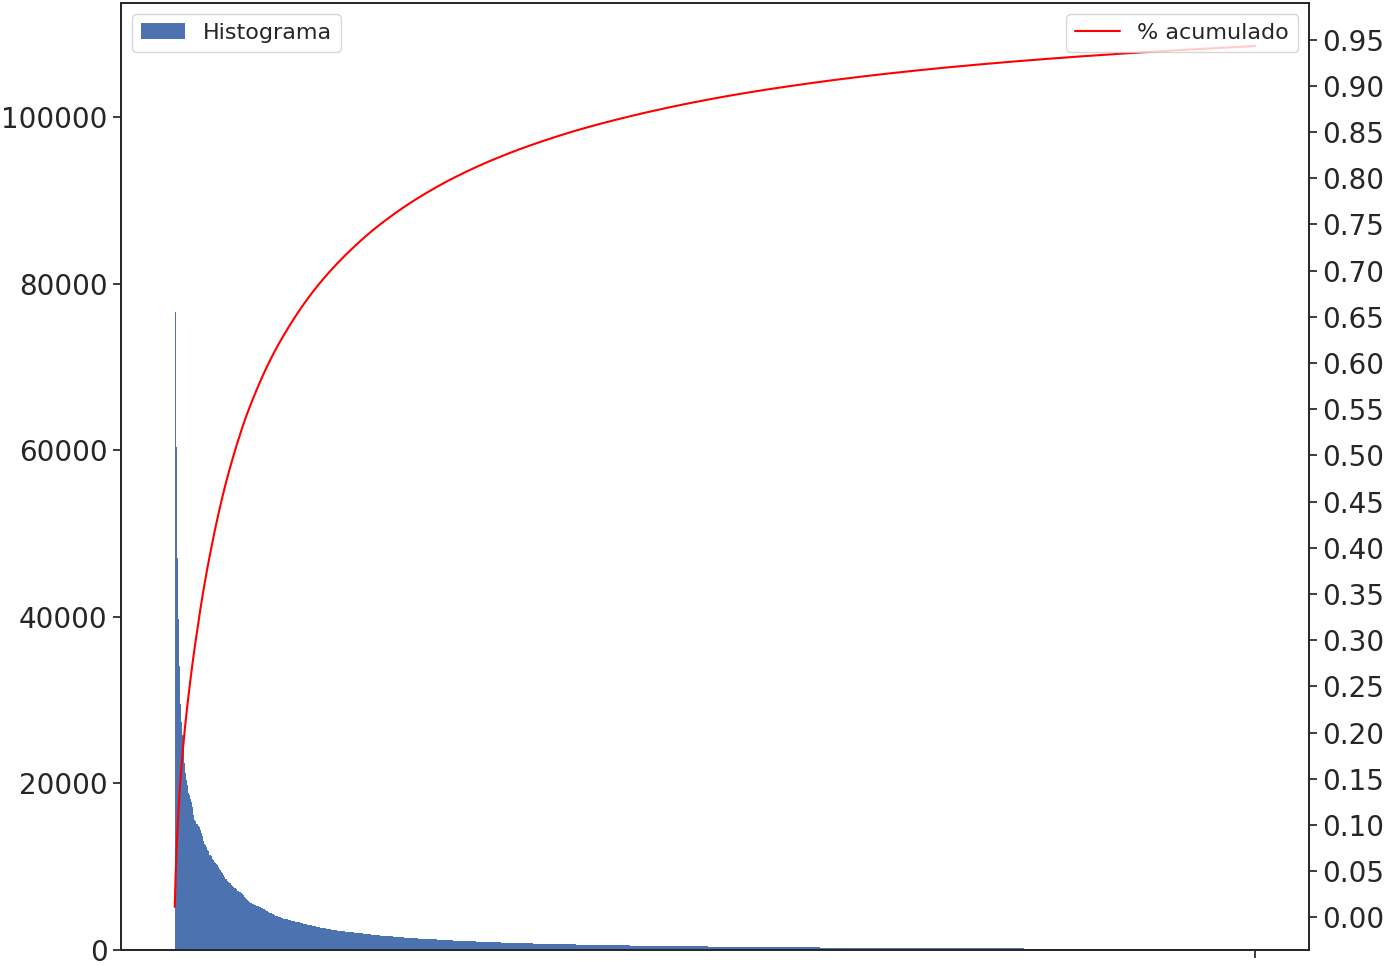
\includegraphics[scale=0.23]{5. Histograma das 5000 primeiras palavras.png}
  \caption{Histograma das primeiras 5000 palavras}
  \label{fig5}
\end{figure}
%--------------------------------------------------------------------------------
\newline\linebreak O histograma evidencia uma cauda muito longa, assim como sugere que não há necessidade (tampouco é recomendado) utilizar toda a base de palavras, uma vez que isso pode prejudicar o treinamento dos algoritmos com palavras com pouca ou nenhuma relevância. Considerou-se, portanto somente as 5.654 palavras que representam 95\% de toda a frequência dos textos, com objetivo de reduzir dimensionalidade e ruídos que pudessem prejudicar o modelo.
%--------------------------------------------------------------------------------
\subsubsection{Classificação dos atendimentos} \label{Sessao4.2.2}
%--------------------------------------------------------------------------------
Realizado o pré-processamento e tratamentos, finalmente pode-se avançar para a classificação. O objetivo era compreender a natureza dos atendimentos para classificá-los entre \textbf{i) dúvida}; \textbf{ii) problema}; \textbf{iii) solicitação}. Essas três classes foram definidas pelas áreas de negócio da empresa, porém essa análise ainda nunca havia sido feita, isto é, não existia uma base rotulada de atendimentos para treinar os modelos. Portanto, a partir dos cerca de 77 mil atendimentos, foi retirada uma amostra de 383 itens para classificação: o tamanho da amostra foi calculado considerando uma margem de erro de 5\% e nível de confiança de 95\%. Estes 383 itens foram rotulados conforme tabela \ref{tab2} e figura \ref{fig6}.
%--------------------------------------------------------------------------------
\begin{table}[!htb]
\caption{Amostra dos atendimentos}
\label{tab2}
\resizebox{\columnwidth}{!}{%
\begin{tabular}{c*{5}{>{$}c<{$}}}
\text{\textbf{Tipo}} & \text{\textbf{Frente atendimento}} & \text{\textbf{Qtde}} & \text{\textbf{Percentual}} & \text{\textbf{Qtde amostra}} \\
Chat & Engajamento N1 & 31.569 & 41,15\% & 158\\
Ticket & Serviço N2 & 20.893 & 27,25\% & 104\\
Ticket & Serviço N1 & 14.917 & 19,46\% & 75\\
Ticket & N3 & 4.823 & 6,29\% & 24\\
Ticket & Avançado & 2.679 & 3,49\% & 13\\
Ticket & Premium & 1.811 & 2,36\% & 9\\
\end{tabular}}
\end{table}
%--------------------------------------------------------------------------------
%--------------------------------------------------------------------------------
\begin{figure}[!htb]
  \centering 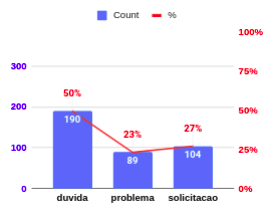
\includegraphics[scale=0.7]{6. Amostra classificada atendimentos.png}
  \caption{Amostra dos atendimentos classificada}
  \label{fig6}
\end{figure}
%--------------------------------------------------------------------------------
\newline\linebreak Para classificação, a amostra foi dividida numa proporção de 70\% treino e 30\% teste e quatro algoritmos foram executados e comparados para identificar o que apresentasse os melhores resultados.
Algumas métricas de validação são comuns para analisar a performance de modelos de classificação, como i) acurácia; ii) valor preditivo negativo; iii) precisão; iv) \emph{recall}; v) especificidade; vi) \emph{F1-score} e vii) área sob a curva ROC; (SCUDILIO, 2020)\cite{SCUDILIO}. Essas métricas são baseadas na matriz de confusão, a partir dos acertos, erros, falsos positivos e falsos negativos do modelo onde, dependendo do objetivo a ser alcançado, cada uma delas contribui de forma diferente na avaliação dos resultados. Uma vez que no caso em questão, buscou-se apenas identificar se o modelo previu corretamente as classes, os falsos positivos e falsos negativos possuem o mesmo peso e, por esse motivo, a métrica de acurácia (\emph{accuracy}) é suficiente para interpretação dos resultados. A tabela \ref{tab3} apresenta os resultados da acurácia dos modelos em seu estado de parâmetros \emph{default}.
%--------------------------------------------------------------------------------
\begin{table}[!htb]
\caption{Classificadores: parâmetros default}
\label{tab3}
\resizebox{\columnwidth}{!}{%
\begin{tabular}{c*{5}{>{$}c<{$}}}
\text{\textbf{Algoritmo}} & \text{\textbf{Train (param default)}} & \text{\textbf{Test (param default)}} \\
Multinomial Naive Bayes Classifier & 60,82\% & 45,69\% \\
Stochastic Gradient Descent Classifier & 100,00\% & 56,90\% \\
C-Support Vector Classification & 97,76\% & 47,41\% \\
Random Forest Classifier & 100,00\% & 50,00\% \\
\end{tabular}}
\end{table}
%--------------------------------------------------------------------------------
\newline\linebreak As colunas “Train” e “Test” (\emph{param default}) representam a acurácia do modelo antes da otimização dos hiperparâmetros (\emph{model tuning}). Para otimização, foram levantadas as possibilidades de combinação de parâmetros de cada um dos algoritmos - que fizessem sentido com o objetivo da análise - e criados \emph{pipelines} para testes com a seleção. A partir disso, portanto, foram usados métodos computacionais para identificar a melhor combinação dos parâmetros, isto é, aqueles que permitem um melhor ajuste e generalização do modelo aos dados.
\newline\linebreak Os métodos utilizados são da Scikit-Learn e consistem em testar, exaustivamente, todas as combinações possíveis dos parâmetros definidos até que a métrica considerada como o indicador de performance (no caso a acurácia), apresente o maior valor nas bases de treino e teste. Por fim, o método também realiza a validação cruzada nas bases de treino e teste conforme a definição de \emph{folds}. Na tabela \ref{tab4}, constam os os mesmos modelos após a otimização dos parâmetros e validação cruzada com 5 \emph{folds}.
%--------------------------------------------------------------------------------
\begin{table}[!htb]
\caption{Classificadores: hiperparâmetros otimizados}
\label{tab4}
\resizebox{\columnwidth}{!}{%
\begin{tabular}{c*{5}{>{$}c<{$}}}
\text{\textbf{Algoritmo}} & \text{\textbf{Test (best param) cross-validation}} & \text{\textbf{Classificação}} \\
Multinomial Naive Bayes Classifier & 60,46\% & 1 \\
Stochastic Gradient Descent Classifier & 63,05\% & 3 \\
C-Support Vector Classification & 58,95\% & 4 \\
Random Forest Classifier & 63,45\% & 2 \\
\end{tabular}}
\end{table}
%--------------------------------------------------------------------------------
\newline\linebreak O classificador escolhido foi o \emph{Multinomial Naive Bayes (NB)}, pois foi o algoritmo que ficou mais equilibrado aos dados, com menor distância de acurácia entre treino e teste, o que não aparenta \emph{overfit}, além de todas as classes terem apresentado resultado similar e satisfatório na predição da classificação (entre treino e teste). Sarkar (2019, p. 298)\cite{SARKAR} cita que “[...] o algoritmo Naive Bayes é usado especificamente para tarefas de predição e classificação tarefas onde temos mais de duas classes” (traduzido pelo autor).  Na figura \ref{fig8}, podemos ver a matriz de confusão do classificador:
%--------------------------------------------------------------------------------
\begin{figure}[!htb]
  \centering 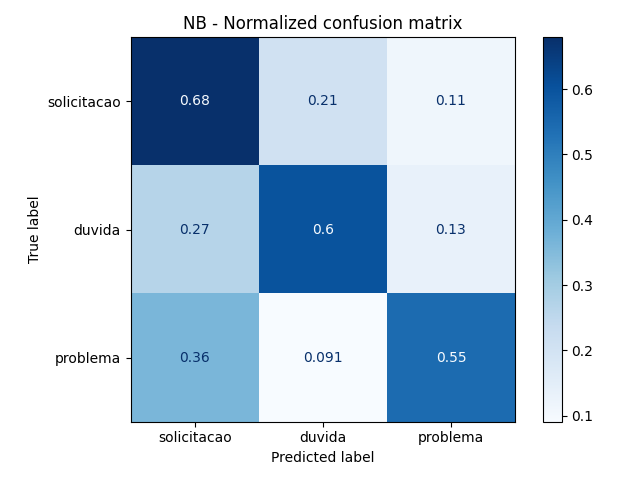
\includegraphics[scale=0.5]{7. Matriz_confusao_NB_normalizada.png}
  \caption{Matriz de confusão normalizada: Naive Bayes Classifier}
  \label{fig7}
\end{figure}
%--------------------------------------------------------------------------------
\newline\linebreak Conforme figura \ref{fig7}, a acurácia final do classificador ficou em 60,46\%. Apesar de não ser ainda um valor tão alto, esta análise não se propõe a ser exaustiva, isto é, ainda existem diversos fatores a serem aprimorados para uso na empresa; porém isso também não impede a continuidade do estudo para que seja possível extrair \emph{insights} iniciais numa primeira observação. Dentre as ações a serem tomadas para melhoria do classificador, provavelmente a aumentar a amostra rotulada para ter uma maior base de treino seja a mais importante como \emph{step 1}.
%--------------------------------------------------------------------------------
\subsection{Combinação dos resultados da clusterização e classificação: primeiros \emph{insights}} \label{Sessao4.4}
%--------------------------------------------------------------------------------
Combinando os resultados dos clientes clusterizados e dos atendimentos classificados, foi possível identificar comportamentos interessantes. Nas figuras \ref{fig8} e \ref{fig9}, podemos verificar que, ainda que a distribuição dos motivos seja unânime entre os grupos - ou seja, duvidas com maior participação, seguido por problema e solicitação - nas dúvidas, o grupo 1 se destaca de forma significativa para mais, enquanto os os grupos 2 e 5 para menos. Interessante notar que o grupo 1 também é o mais volumoso em número de clientes; ao passo em que os grupos 2 e 5 estão entre os menos volumosos (vide figura \ref{fig4}).
%--------------------------------------------------------------------------------
\begin{figure}[!htb]
  \centering 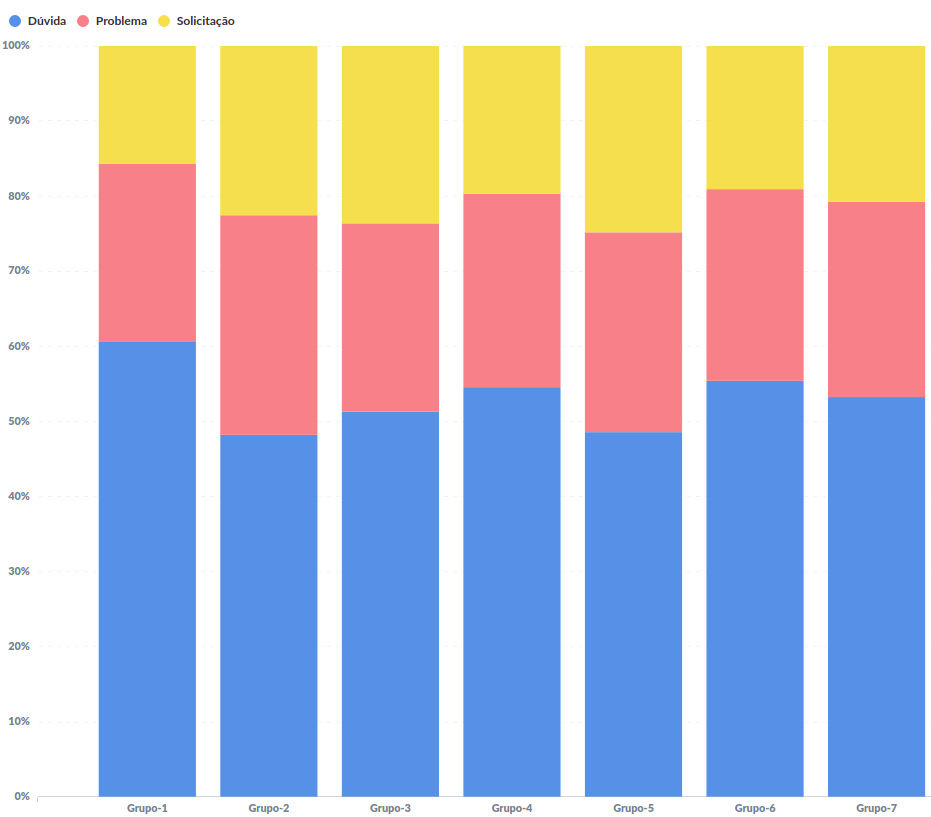
\includegraphics[scale=0.35]{8. Classificação atendimentos (7 clusters) - chart.png}
  \caption{Distribuição das classes pelos grupos}
  \label{fig8}
\end{figure}
%--------------------------------------------------------------------------------
%--------------------------------------------------------------------------------
\begin{figure}[!htb]
  \centering 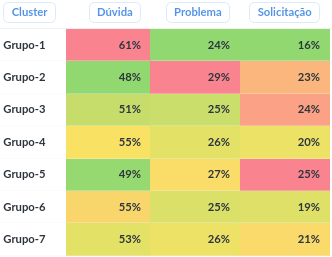
\includegraphics[scale=0.7]{9. Classificação atendimentos (7 clusters) - table.png}
  \caption{Mapa de calor das classes pelos grupos}
  \label{fig9}
\end{figure}
%--------------------------------------------------------------------------------
\newline\linebreak Já na figura \ref{fig10}, podemos notar que os grupos 1, 4 e 6 apresentam uma taxa de contato menor do que os demais, ou seja, geram menos demanda no atendimento para a companhia. Também é interessante observar que os grupos com maiores taxas de contato (2, 3, 5 e 7) também apresentam o volume de “solicitações” maior que os demais.
%--------------------------------------------------------------------------------
\begin{figure}[!htb]
  \centering 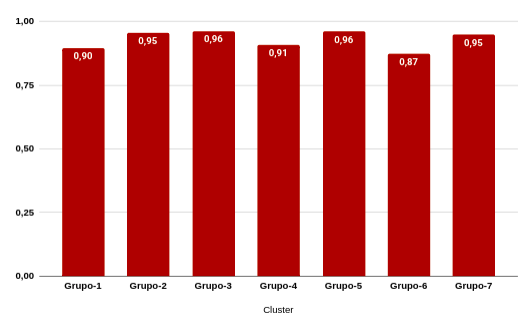
\includegraphics[scale=0.6]{10. Concat rate (7 clusters).png}
  \caption{Taxa de contato (contact rate) por grupo}
  \label{fig10}
\end{figure}
%--------------------------------------------------------------------------------
\section{Conclusão} \label{Sessao5}
Com a análise dos resultados, realizada no item \ref{Sessao4.4}; fica evidente que existe distinção entre os tipos de clientes da empresa e na forma como estes interagem os com ela, o que era uma das questões centrais a serem respondidas por meio deste estudo.
Por meio dos resultados da etapa 1 (clusterização - \ref{Sessao4.1}), foi possível verificar que a maioria das variáveis consideradas apresentaram comportamentos diferentes para cada um dos 7 grupos, o que implica na inferência de que foram úteis na separação desses clientes, permitindo compreender o que é relevante nessa separação, bem como identificar e traçar perfis para os grupos e os clientes que fazem parte deles.
Já na etapa \ref{Sessao4.2.1}, a partir da classificação dos atendimentos, verificou-se que as dúvidas são o maior motivo de contato dos clientes com a empresa, sendo cerca de metade deles. A outra parte, se divide também de forma similar entre as duas demais categorias (problema e solicitação). Ou seja, fica evidente que para reduzir o volume de atendimentos demandados, o foco inicial da empresa deve ser na redução das dúvidas. Importante considerar, no entanto, que essa proporção varia entre os grupos, o que também era uma questão central a ser compreendida. Essa interpretação sugere que os tipos de clientes (perfis) possuem demandas diferentes e, desta forma, ações específicas podem ser necessárias para cada grupo.
A pesquisa, no entanto, não é exaustiva e não se propôs a esgotar o assunto, mas sim em dar um primeiro passo, obter \emph{insights} e identificar critérios que permitissem compreender os perfis de clientes e a relação destes com os tipos de demandas que fazem no atendimento \emph{(service-desk)}. Isto é, criar uma metodologia inicial de análise para que a empresa possa entender a jornada de seus clientes e elaborar ações, seja de processos ou tecnologia, que melhorem a experiência.
A partir dos resultados, cabe como próximos passos uma extensa análise exploratória, considerando as demais variáveis utilizadas na clusterização dos clientes em conjunto com as áreas de negócio da empresa, para melhor a interpretação e assim enfim, colaborar na nos planos de ação a serem formulados e no desenvolvimento do negócio, seja na experiência do cliente, ou na melhora de eficiência da companhia, via alavancagem operacional do seu time de atendimento, com automação de rotinas repetitivas ou que agregam pouco valor a companhia e ao cliente.
%--------------------------------------------------------------------------------

\begin{thebibliography}{99}
  \bibliographystyle{unsrt}

\bibitem{SCHMIDT} SCHMIDT, Jose Luiz dos Santos e Paulo. 
    \textit{História da Contabilidade: foco na evolução das escolas do pensamento contábil.} Santos: Atlas, 2008. 176 p.

\bibitem{NEGRA} NEGRA, Elizabete Marinho Serra.
    \textit{Evidências das partidas dobradas através da Matemática na Mesopotâmia.} Revista do CRC/PR, Curitiba, 2003.

\bibitem{IMPERATORE} IMPERATORE, Simone Loureiro Brum.
    \textit{Fundamentos da Contabilidade.} Curitiba: Intersaberes, 2017. 173 p.

\bibitem{ISTOE} ISTOÉ DINHEIRO.
    \textit{Tecnologia - Contabilidade Digital: escritórios contábeis on-line ganham espaço com modelo de startup e promessa de custos menores.} 2020.

\bibitem{EXAME} EXAME.
    \textit{Informalidade atinge 98\% das pequenas empresas.} 2008.

\bibitem{SHAIKH} SHAIKH, Raheel.
    \textit{Choosing the right Encoding method-Label vs OneHot Encoder.} Towards Data Science, 2018.

\bibitem{SCIPY} Scipy.
    \textit{Cluster Hierarchy Linkage.} Scipy Python Library, 2020.

\bibitem{SARKAR} SARKAR, Dipanjan.
    \textit{Text Analytics with Python: a practitioner's guide to natural language processing.} 2. ed. Bangalore, Karnataka, India: Apress, 2019. 668 p.

\bibitem{BOEHMKE} BOEHMKE, Bradley.
    \textit{Business Analytics R Programming Guide: creating text features with bag-of-words, n-grams, parts-of-speach and more.} University of Cincinnati, 2020.

\bibitem{SCUDILIO} SCUDILIO, Juliana.
    \textit{Qual a melhor métrica para avaliar os modelos de Machine Learning?} Flai Inteligência Artificial, 2020.

\bibitem{SEIDEL} SEIDEL, Enio Júnior et al.
    \textit{Comparação entre o método Ward e o método K-médias no agrupamento de produtores de leite.} Santa Maria, 2008.

\end{thebibliography}
\end{document}
